% !TEX encoding = UTF-8 Unicode
\chapter{Sprint 1 - File Processing}

\begin{figure}[h]
    \begin{center}
        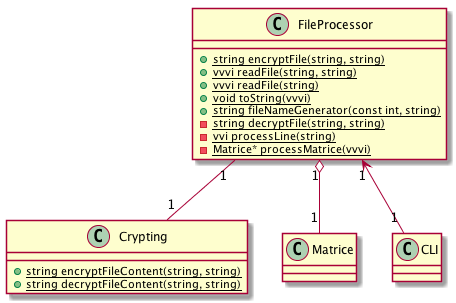
\includegraphics[scale=0.40]{./ressources/graph/FileProcessor.png}
    \end{center}
    \caption{Class diagram}
    \label{Solution - FileProcessing class diagram}
\end{figure}
\bigskip


\section{Matrice format}

In order to have a simple lecture of the plain text file representing a 2 dimensional matrix, with the possibility of
having matrix item of greater dimensions.

\begin{figure}[h]
	\begin{minipage}{0.25\textwidth}
	\flushleft
	Simple 2D Matrix
	\centering
		\begin{verbatim}
		255 255 155
		156 156 157
		255 255 255
		\end{verbatim}
	\end{minipage}
\hfill
\noindent
	\begin{minipage}{0.45\textwidth}
	\flushright
	2D Matrix with multi-dimensional value
		\centering
		\begin{verbatim}
		255,255,255 255,255,255 155,155,155
		156,255,255 156,255,255 157,255,255
		255,255,255 255,255,255 255,255,255
		\end{verbatim}
	\end{minipage}
\label{fig:Plain text matrix format}
\end{figure}

\section{Crypting}

One of the required features was to being handle the case of cipher file.\\
The amount of algorithm and their variants, required us for this project to select a proper and simple crypting method for the:w matrix file the user would used.\\
A decrypting method, but also a crypting method should be developed in order to process properly both plain text and cipher file.

\par
Different crypto libraries have been tested for this features :
\begin{itemize}
	\item openssl
	\item botan
\end{itemize}

\par
First tests with OpenSSL library didn't gave result. The library is low-level, bad-documented and complexify too much the process of encryption and decryption of a file, while for this above feature we were mostly looking for a simple and quick way.

\par
Second test with Botan library gave usefull result. The library is easily accessible (while it still need some cryptographic knowledges to quickly handle availables features).\\
Among the available algorithms (Serpent, AES, Blowfish,etc.) AES-256 has been selected for its broad usage and simplicity.


\section{FileProcessor}

FileProcessor class handle the reading method for both plain text file and cipher file.\\
This class should store the content of user 2D matrix file into a simple data structure (vector), and
give an access the Matrice class which will handle the complexe structure construction algorithm.\\
It also handle the usage of encryption and decryption methods.

\par
FileProcessor class should be the interface between the file selected by the User and the construction of a complexe
matrix data structure.